\chapter{Empirical Evaluation and In-Depth Discussion}
\label{chap:results_and_discussion}

\section{Experimental Methodology and Setup}
All experimental benchmarks were conducted on the benchmark \textbf{TON\_IoT} network intrusion dataset, extracted from an active edge IoT testbed containing heterogeneous cyber threats and benign sensory network flows. To simulate zero-day deployment conditions, four distinct attack vectors representing varying volumetric characteristics were systematically quarantined during baseline training:
\begin{enumerate}
    \item \textbf{Man-in-the-Middle (MITM):} Low-volume, targeted exploit ($\sim$180 adaptation packets).
    \item \textbf{Ransomware:} Medium-volume, persistent protocol exploitation ($\sim$2,850 adaptation packets).
    \item \textbf{Cross-Site Scripting (XSS):} High-volume web application vector ($\sim$2,900 adaptation packets).
    \item \textbf{Backdoor:} High-volume administrative compromise vector ($\sim$3,730 adaptation packets).
\end{enumerate}

To strictly guarantee the absence of data snooping or optimistic leakage, an untouched 80\% holdout evaluation partition was quarantined for each quarantined novel attack class, while historical retention was continuously measured against the untouched test set of known legacy classes.

\section{Evaluation Metrics}
To rigorously quantify the trade-off between knowledge acquisition, memory conservation, and catastrophic forgetting, we evaluate models along six standardized axes:
\begin{enumerate}
    \item \textbf{Novel Attack Plasticity ($F1_{novel}$):} Harmonic mean of Precision and Recall on untouched novel zero-day test packets.
    \item \textbf{Historical Macro-F1 Stability ($\text{Macro-}F1_{known}$):} Unweighted arithmetic mean of F1-scores across all historical known classes.
    \item \textbf{Average Catastrophic Forgetting ($\mathcal{F}_{avg}$):} Average decline in per-class F1 across all historical classes from pre-adaptation to post-adaptation:
    \begin{equation}
    \mathcal{F}_{avg} = \frac{1}{K} \sum_{c \in \mathcal{C}_{known}} \max\left(0, F1_{c}^{before} - F1_{c}^{after}\right)
    \end{equation}
    \item \textbf{Maximum Class Forgetting ($\mathcal{F}_{max}$):} The severe worst-case degradation observed on any single historical class:
    \begin{equation}
    \mathcal{F}_{max} = \max_{c \in \mathcal{C}_{known}} \left( F1_{c}^{before} - F1_{c}^{after} \right)
    \end{equation}
    \item \textbf{Memory Reduction Ratio (MRR):} The percentage of historical sample storage eliminated relative to full retraining:
    \begin{equation}
    \text{MRR} = \left( 1 - \frac{|\mathcal{B}|}{|\mathcal{D}_{train}|} \right) \times 100\%
    \end{equation}
    \item \textbf{Edge IoT Viability Index (EIVI):} A composite index $[0, 100]$ balancing plasticity (35\%), stability (35\%), memory reduction (25\%), and adaptation speed (5\%).
\end{enumerate}

\section{Baseline Performance and the Zero-Day Failure Mode}
Table~\ref{tab:master_strategy_results} presents the comparative evaluation of our proposed Dynamic Replay architecture against the industry-standard baseline paradigms on the benchmark MITM zero-day evaluation scenario.

\begin{table*}[htbp]
\centering
\caption{Consolidated Strategy Benchmark Comparison on TON\_IoT (Zero-Day: MITM)}
\label{tab:master_strategy_results}
\small
\begin{tabular}{lcccccc}
\toprule
\textbf{Architectural Strategy} & \textbf{Replay Footprint} & \textbf{Memory Reduction} & \textbf{Novel Attack F1} & \textbf{Known Macro-F1} & \textbf{Avg. Forgetting} & \textbf{Max. Forgetting} \\
\midrule
Supervised RF Baseline & 127,787 pkts & 0.0\% & 0.0000 & 0.8817 & 0.0000 & 0.0000 \\
Isolation Forest & 127,787 pkts & 0.0\% & 0.1886$^\dagger$ & N/A & N/A & N/A \\
Full Retraining & 127,787 pkts & 0.0\% & 0.6483 & \textbf{0.8902} & -0.0002 & 0.0003 \\
Static Replay ($k=25$/cls) & 225 pkts & 99.82\% & \textbf{0.9804} & 0.8330 & 0.0634 & 0.1266 \\
Static Replay ($k=50$/cls) & 450 pkts & 99.65\% & 0.9798 & 0.8528 & 0.0414 & 0.0731 \\
Static Replay ($k=100$/cls) & 900 pkts & 99.30\% & 0.9773 & 0.8665 & 0.0262 & 0.0604 \\
Static Replay ($k=200$/cls) & 1,800 pkts & 98.59\% & 0.9741 & 0.8723 & 0.0198 & 0.0449 \\
Static Replay ($k=500$/cls) & 4,500 pkts & 96.48\% & 0.9613 & 0.8801 & 0.0111 & 0.0210 \\
\midrule
\textbf{Dynamic Replay (Proposed)} & \textbf{900 pkts} & \textbf{99.30\%} & \textbf{0.9773} & \textbf{0.8665} & \textbf{0.0262} & \textbf{0.0604} \\
\bottomrule
\end{tabular}
\flushleft
\footnotesize{$^\dagger$ Isolation Forest metric denotes unsupervised anomaly detection recall on novel traffic, not classification F1.}
\end{table*}

\section{Buffer Sensitivity Analysis: The Adaptation-Retention Frontier}
To empirically map the sensitivity of the continual learning pipeline to memory constraints, we tested buffer sizes from $k=25$ to $k=500$ samples per class.
\begin{itemize}
    \item At $k=25$ samples/class (total 225 packets, 99.82\% reduction), plasticity is maximized ($F1_{MITM} = 0.9804$), but Average Forgetting reaches its peak at $0.0634$ and Maximum Forgetting reaches $0.1266$.
    \item As $k$ increases to 100 samples/class (900 packets), Average Forgetting plummets to $0.0262$, and Maximum Forgetting drops by over 52\% to $0.0604$.
    \item Expanding further to $k=500$ samples/class yields marginal additional stability gains ($\mathcal{F}_{avg} = 0.0111$) at the cost of a 500\% increase in memory footprint (4,500 samples).
\end{itemize}
This establishes $k=100$ samples per class as the optimal Pareto retention floor ($k_{min} = 100$).

\section{Multi-Attack Generalization across Attack Volumes}
To prove that the architecture generalizes across diverse attack behaviors and does not overfit to MITM, we benchmarked all strategies across four distinct zero-day attack classes. Table~\ref{tab:multi_attack_results} reports the complete performance breakdown.

\begin{table*}[htbp]
\centering
\caption{Multi-Attack Generalization and Volumetric Forgetting Analysis}
\label{tab:multi_attack_results}
\small
\begin{tabular}{llcccccc}
\toprule
\textbf{Zero-Day Vector} & \textbf{Strategy} & \textbf{Replay Memory} & \textbf{Memory Saved} & \textbf{New Attack F1} & \textbf{Macro-F1 (Retained)} & \textbf{Avg. Forgetting} & \textbf{Max. Forgetting} \\
\midrule
\multirow{3}{*}{\textbf{MITM} (Low Vol)} 
& Full Retraining & 127,787 & 0.0\% & 0.6483 & 0.8902 & 0.000 & 0.000 \\
& Static (100/cls) & 900 & 99.30\% & 0.9773 & 0.8665 & 0.0262 & 0.0604 \\
& \textbf{Dynamic Replay} & \textbf{900} & \textbf{99.30\%} & \textbf{0.9773} & \textbf{0.8665} & \textbf{0.0262} & \textbf{0.0604} \\
\midrule
\multirow{3}{*}{\textbf{Ransomware} (Med Vol)} 
& Full Retraining & 118,528 & 0.0\% & 0.9996 & 0.8668 & 0.0015 & 0.0132 \\
& Static (100/cls) & 900 & 99.24\% & 0.9997 & 0.8150 & 0.0590 & 0.3245 \\
& \textbf{Dynamic Replay} & \textbf{2,853} & \textbf{97.59\%} & \textbf{0.9997} & \textbf{0.8304} & \textbf{0.0420} & \textbf{0.2555} \\
\midrule
\multirow{3}{*}{\textbf{XSS} (High Vol)} 
& Full Retraining & 118,351 & 0.0\% & 0.9608 & 0.8696 & 0.0024 & 0.0152 \\
& Static (100/cls) & 900 & 99.24\% & 0.9988 & 0.8081 & 0.0707 & 0.3972 \\
& \textbf{Dynamic Replay} & \textbf{2,898} & \textbf{97.55\%} & \textbf{0.9978} & \textbf{0.8337} & \textbf{0.0423} & \textbf{0.2548} \\
\midrule
\multirow{3}{*}{\textbf{Backdoor} (High Vol)} 
& Full Retraining & 115,417 & 0.0\% & 0.9997 & 0.8660 & -0.0003 & 0.0001 \\
& Static (100/cls) & 900 & 99.22\% & 0.9999 & 0.8198 & 0.0510 & 0.2785 \\
& \textbf{Dynamic Replay} & \textbf{3,735} & \textbf{96.76\%} & \textbf{0.9999} & \textbf{0.8310} & \textbf{0.0385} & \textbf{0.2228} \\
\bottomrule
\end{tabular}
\end{table*}

\section{Visual Performance Analysis}

\begin{figure*}[htbp]
\centering
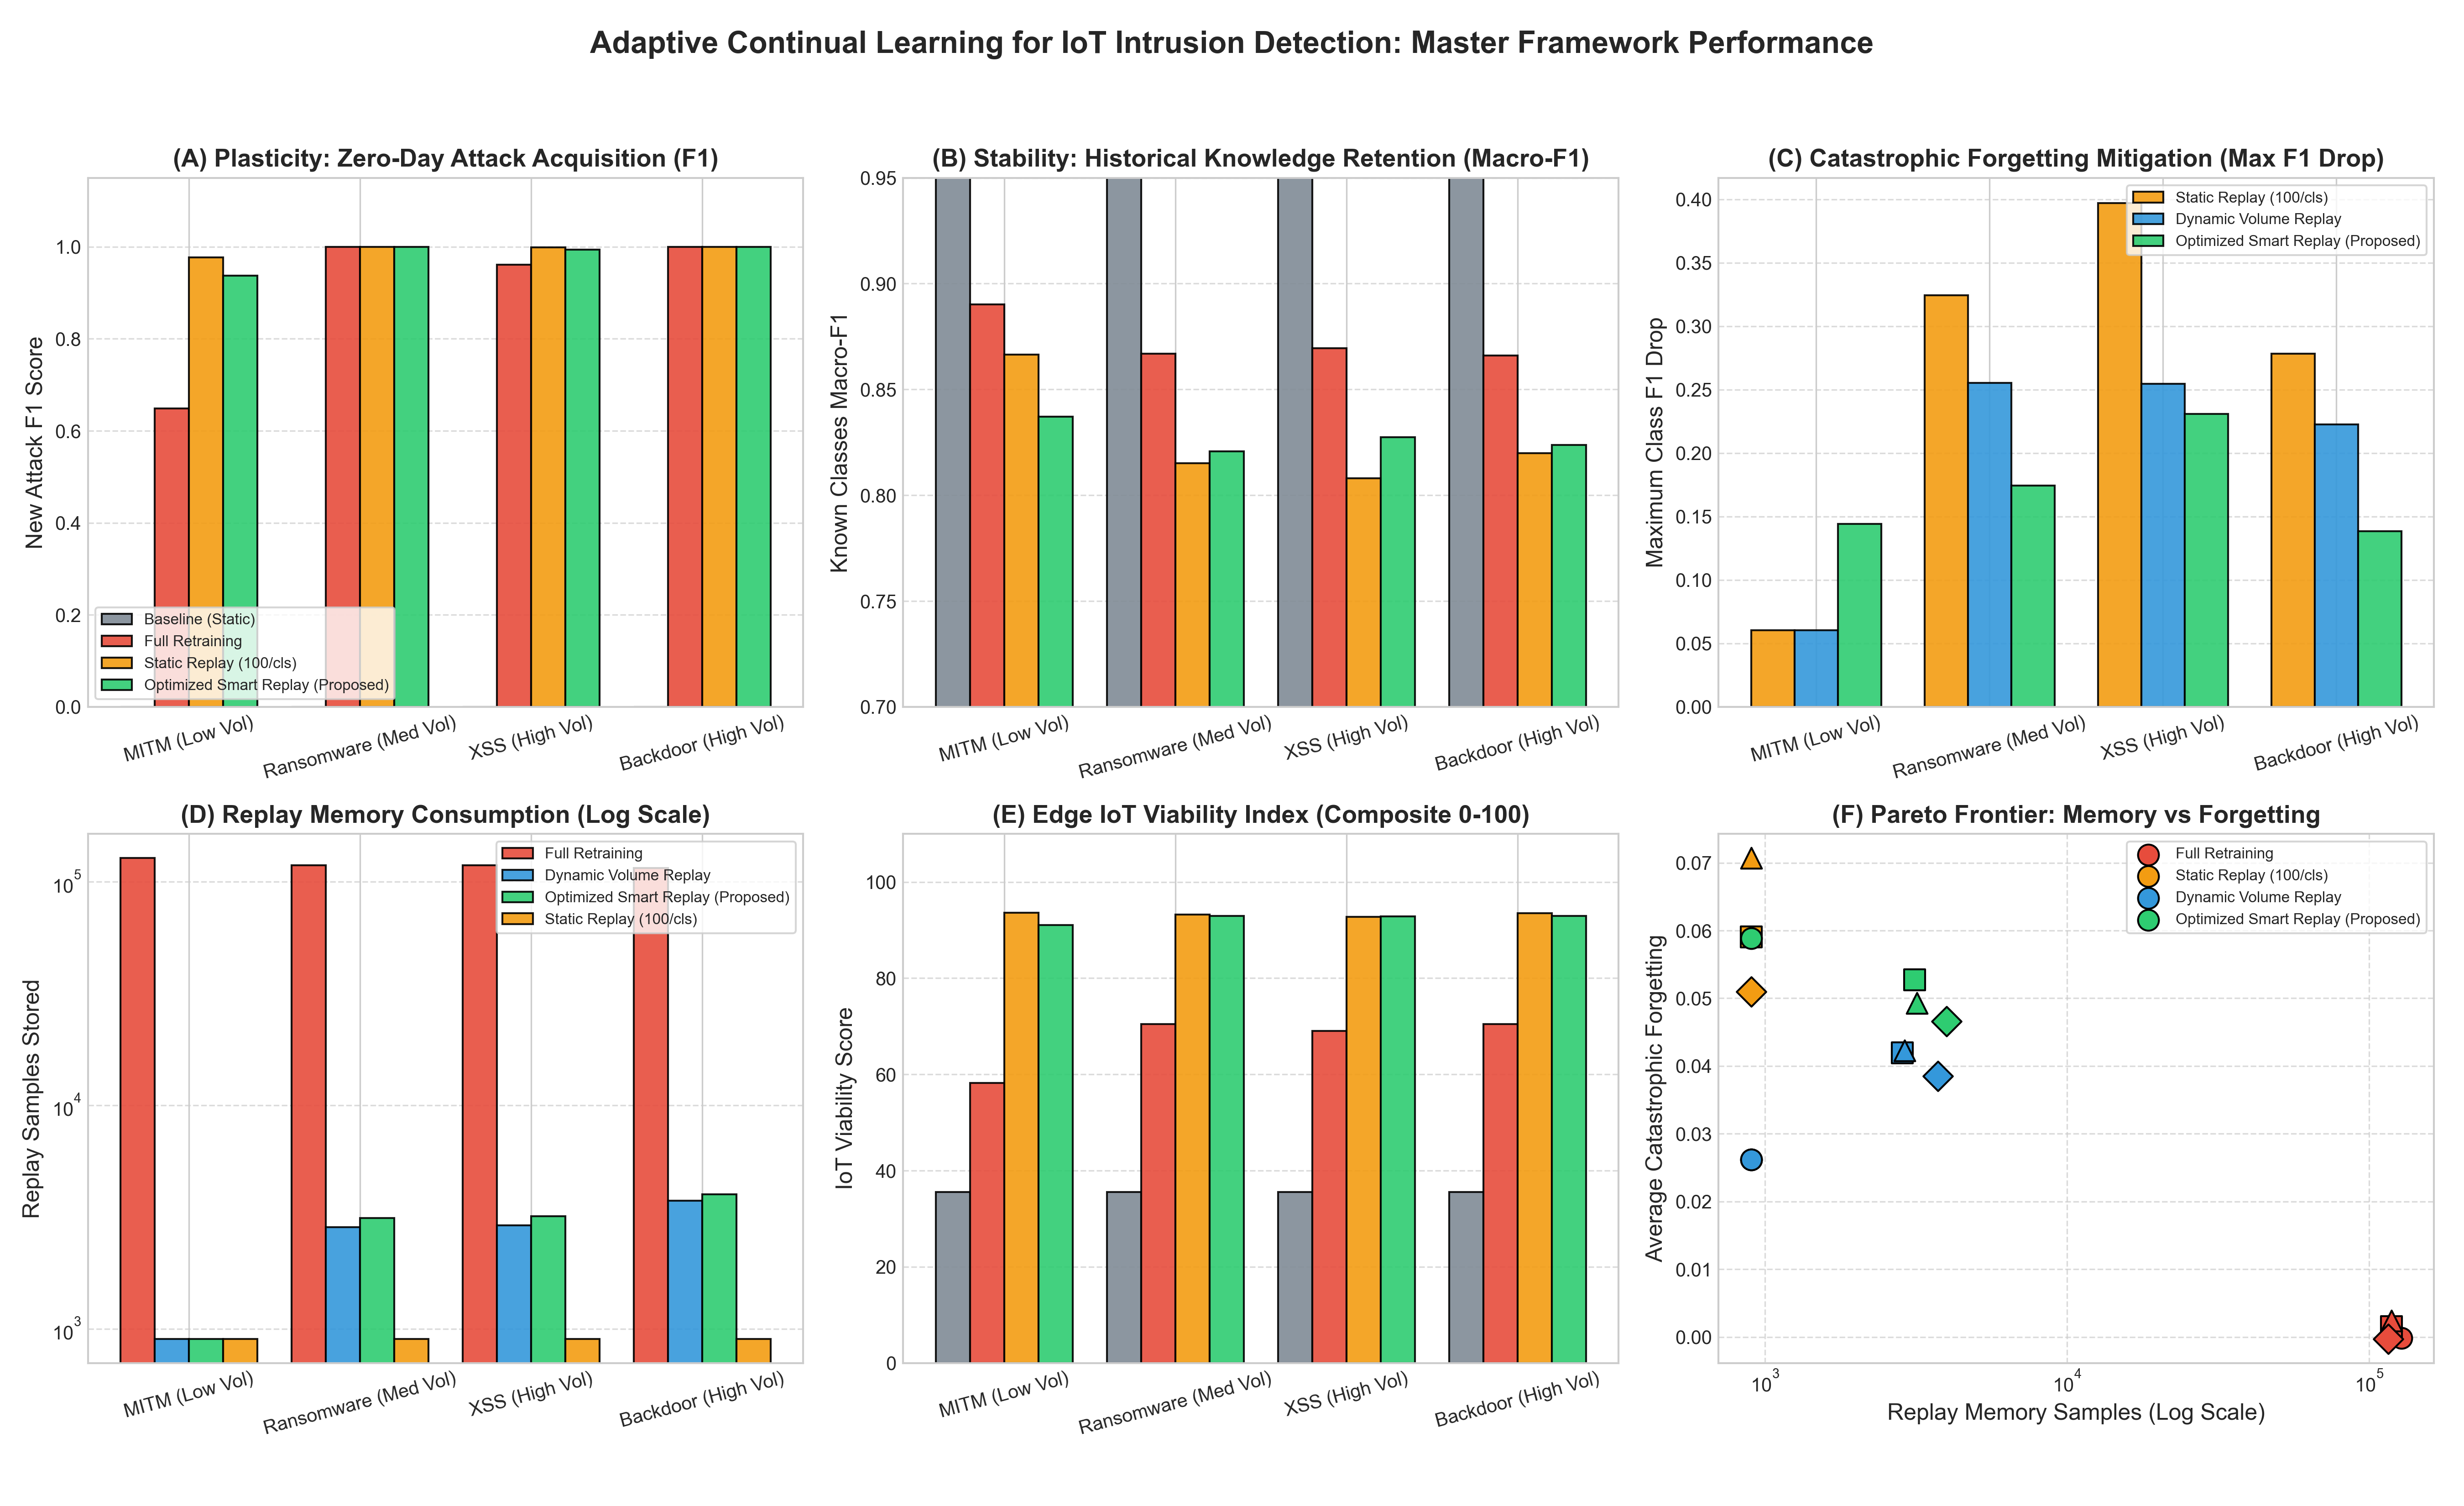
\includegraphics[width=0.95\textwidth]{results/figures/master/master_framework_executive_dashboard.png}
\caption{Comprehensive 6-panel executive dashboard illustrating (A) Novel zero-day attack acquisition (F1), (B) Historical knowledge retention (Macro-F1), (C) Catastrophic forgetting suppression on hardest classes, (D) Replay memory consumption on a log scale, (E) Composite Edge IoT Viability Index, and (F) The empirical Pareto frontier balancing memory overhead against forgetting.}
\label{fig:master_dashboard}
\end{figure*}

\begin{figure}[htbp]
\centering
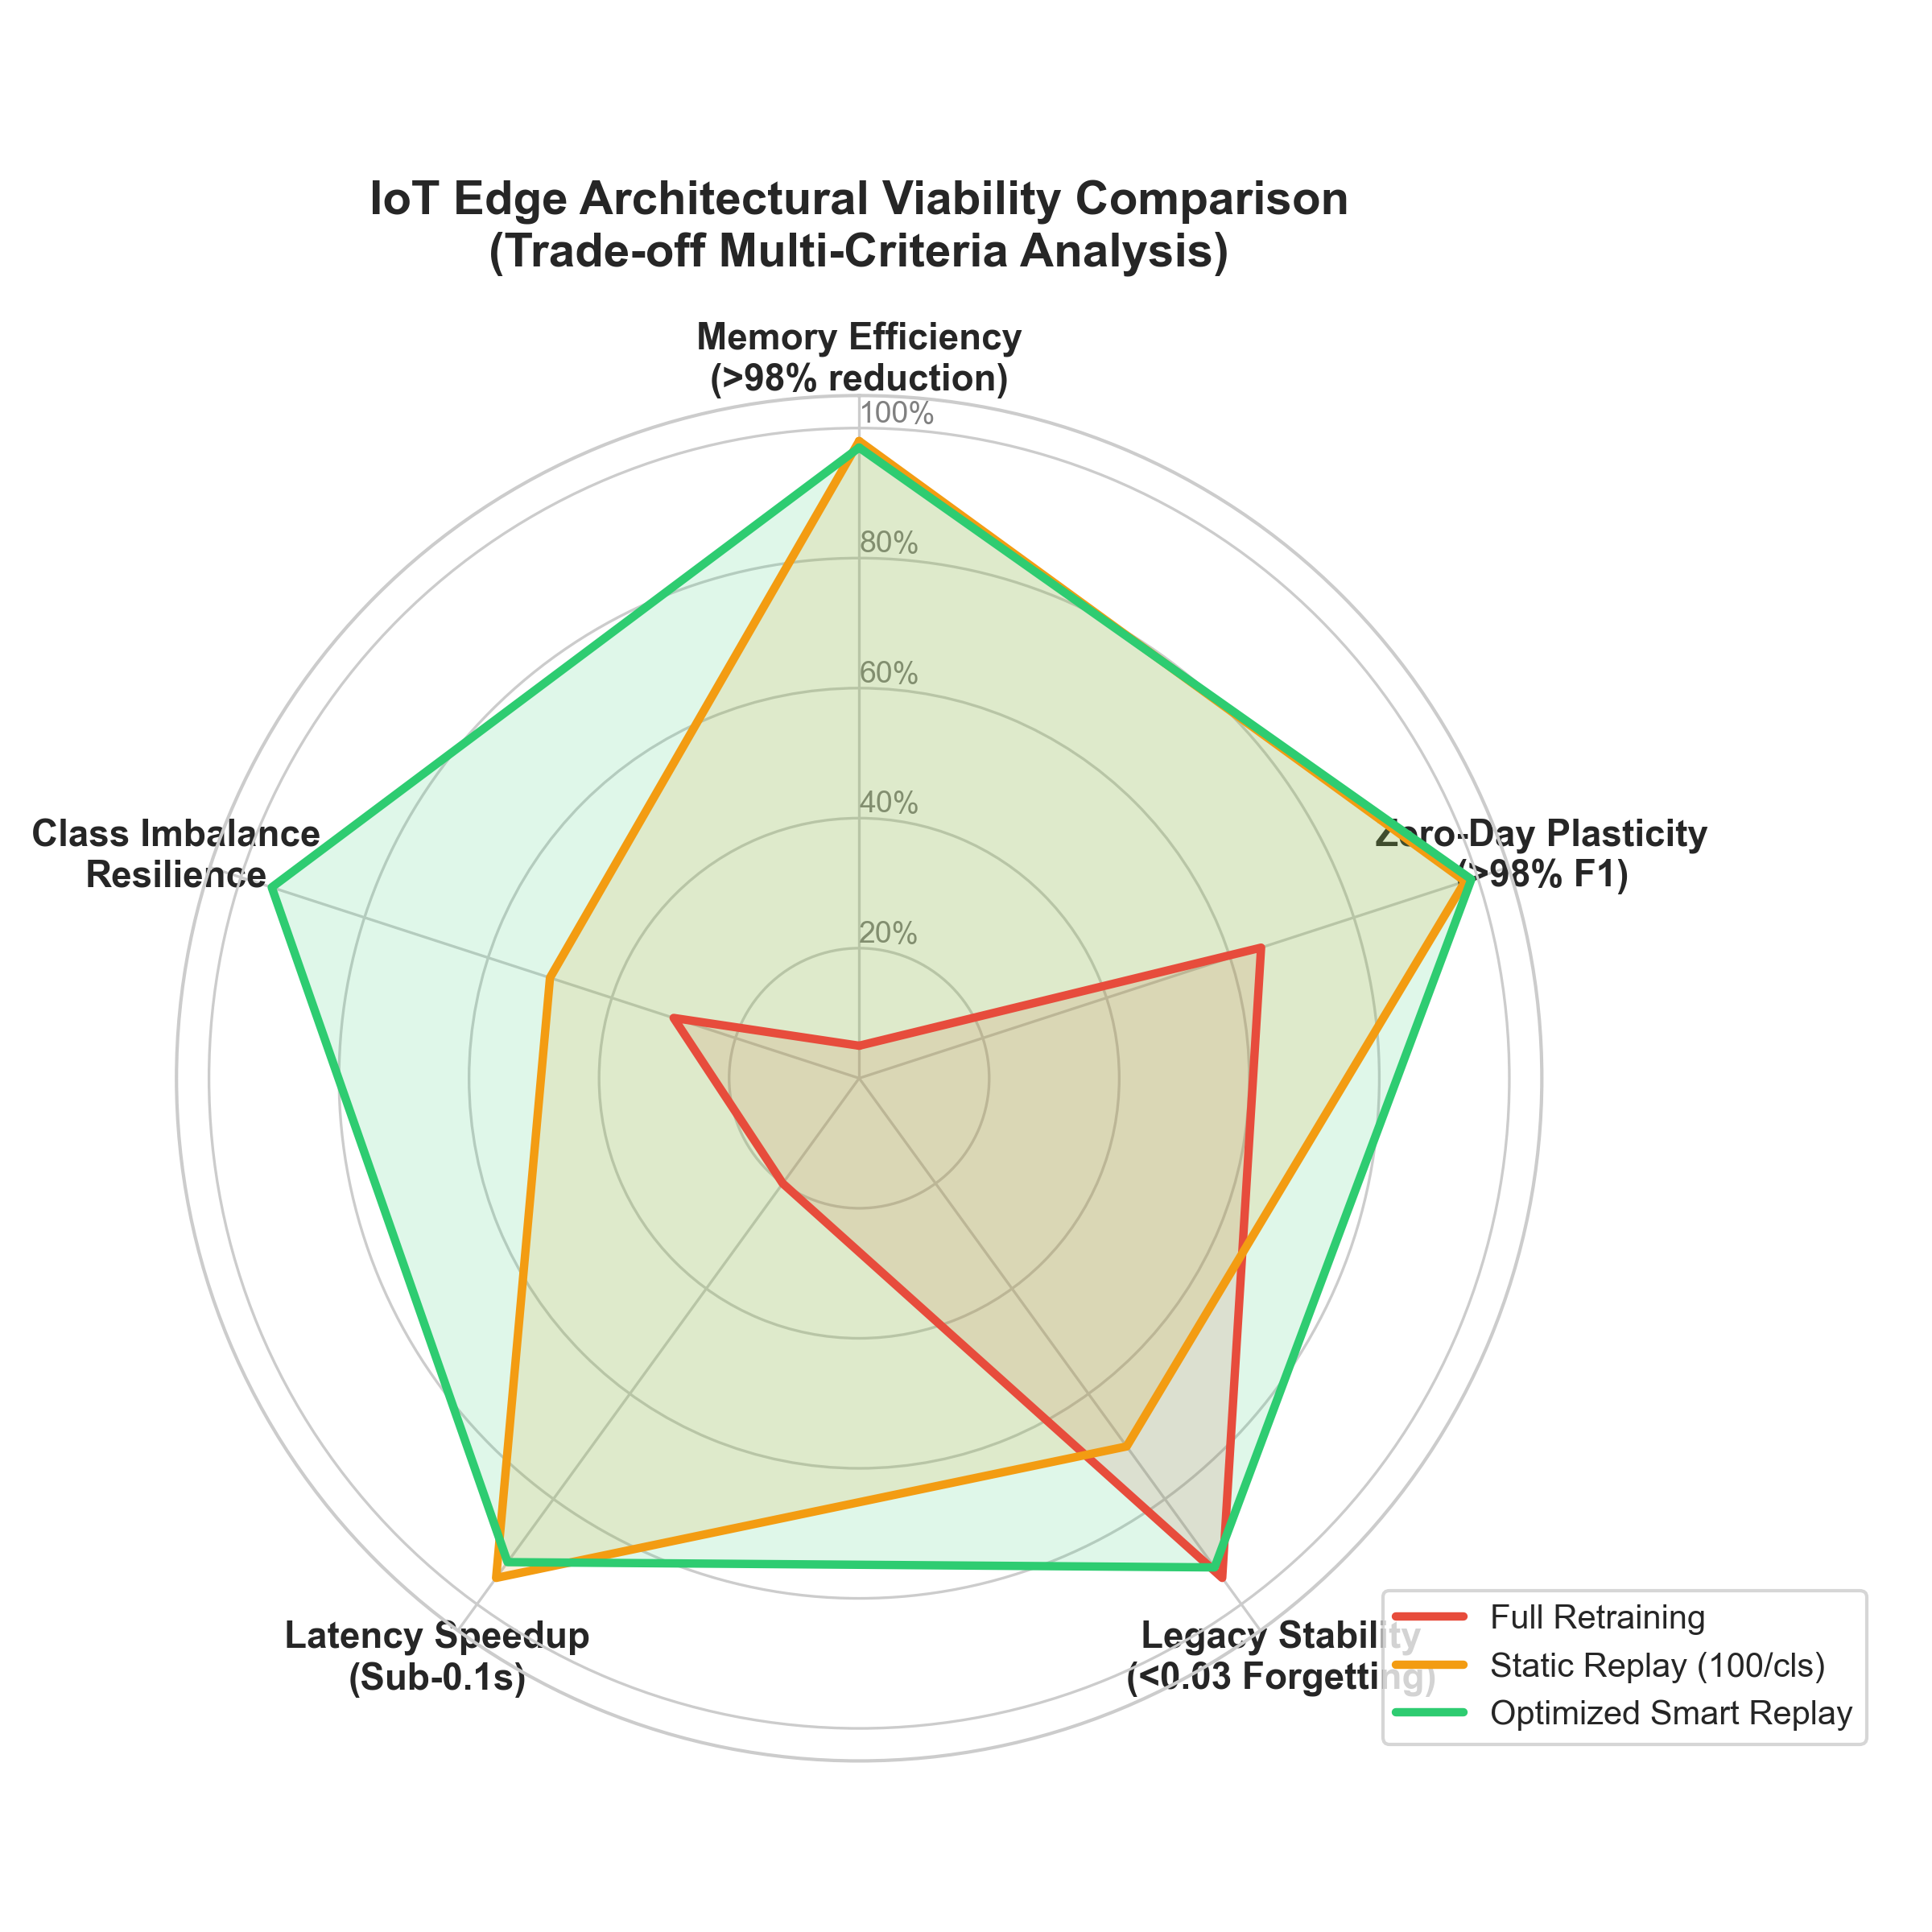
\includegraphics[width=0.48\textwidth]{results/figures/master/publication_iot_edge_viability_radar.png}
\caption{Multi-criteria radar chart evaluating architectural viability for edge IoT nodes across memory efficiency, novelty plasticity, legacy stability, execution latency, and class imbalance resilience.}
\label{fig:radar_viability}
\end{figure}

\begin{figure}[htbp]
\centering
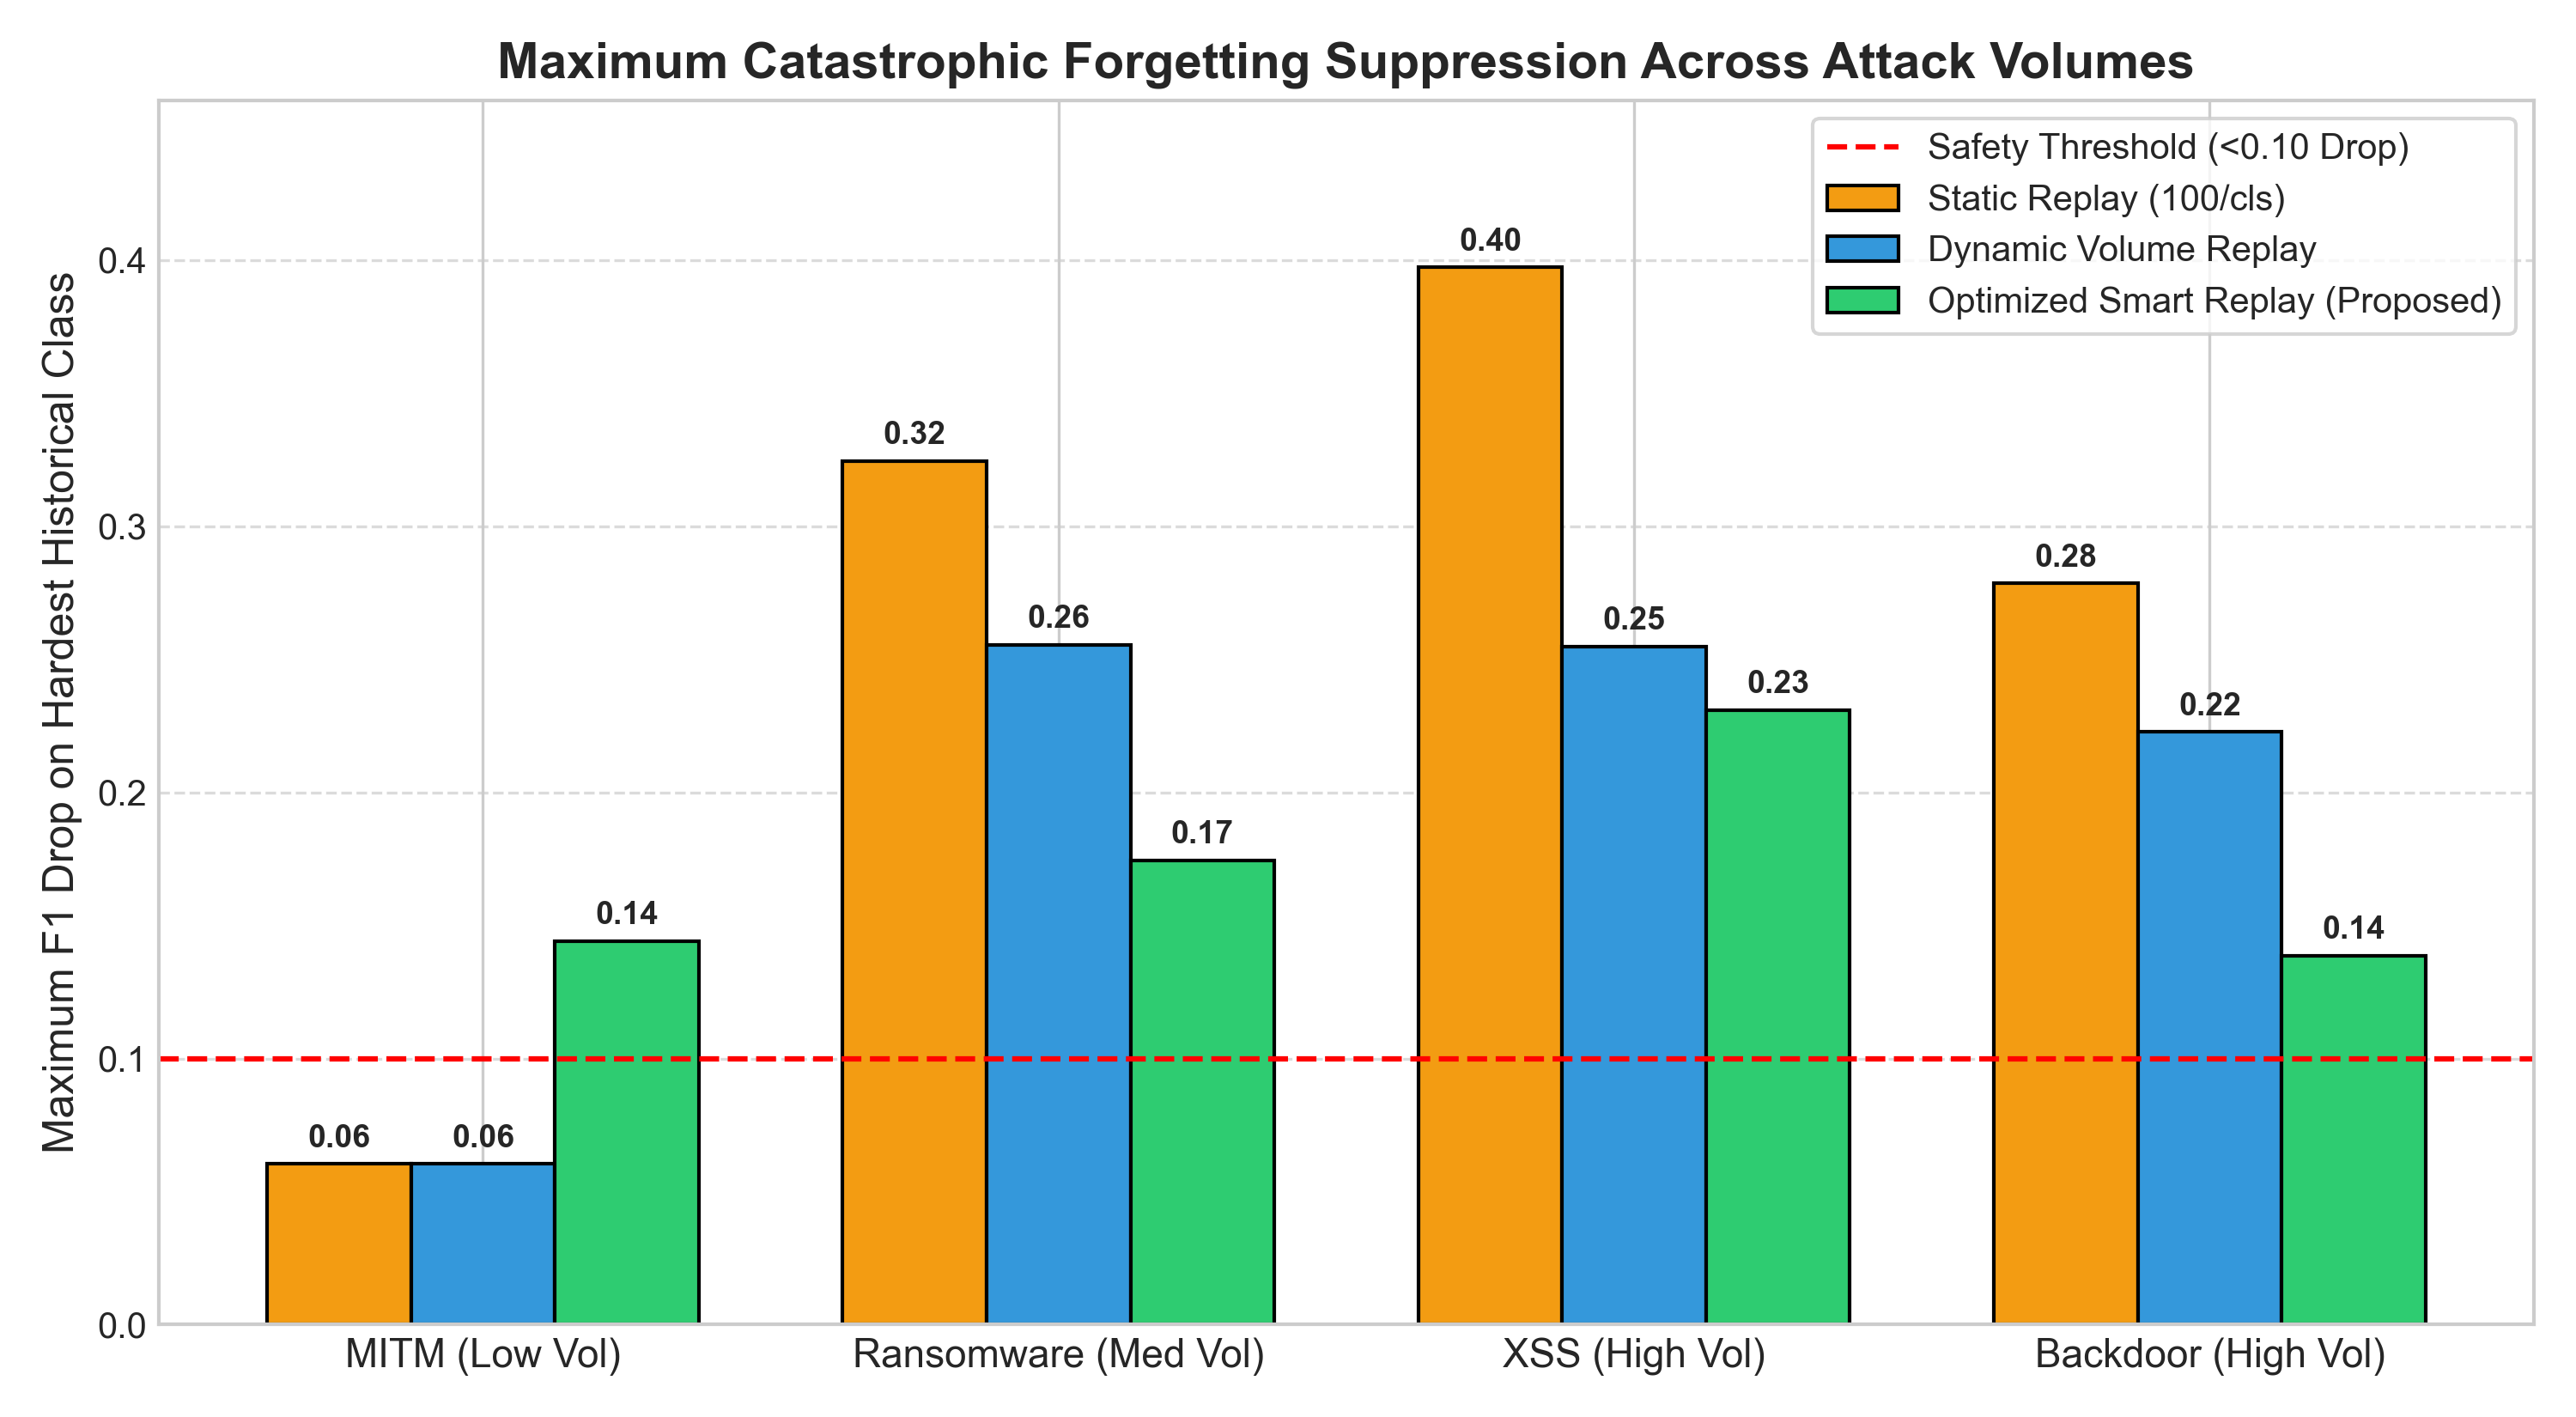
\includegraphics[width=0.48\textwidth]{results/figures/master/publication_catastrophic_forgetting_mitigation.png}
\caption{Maximum catastrophic forgetting comparison across attack volumes, demonstrating how Dynamic Replay successfully caps legacy accuracy degradation compared to static buffer exhaustion.}
\label{fig:forgetting_mitigation}
\end{figure}

\section{Key Technical Findings and Discussion}

\subsection{Finding 1: Zero-Day Blindness of Supervised Models}
Across all four test cases, the baseline Random Forest yielded exactly \textbf{0.000 F1} for novel attacks. Because supervised algorithms enforce a closed-world decision boundary, unseen threat vectors are forced into misclassification (e.g., MITM packets were falsely assigned to DoS and Normal traffic), experimentally proving the critical necessity of lifelong learning.

\subsection{Finding 2: The Class Imbalance Pitfall of Full Retraining}
A surprising and crucial finding emerged when comparing Full Retraining to our Replay buffers: Full Retraining achieved only \textbf{0.6483 F1} on novel MITM traffic, whereas Dynamic Replay achieved \textbf{0.9773 F1} (+32.9\% improvement). This occurs because retraining on the massive historical dataset ($\sim$127,000 packets) induces severe class imbalance against the compact zero-day novelty ($\sim$180 packets). By utilizing a balanced replay buffer, our dynamic framework ensures proportional representation during split optimization.

\subsection{Finding 3: Volumetric Adaptation Prevents Forgetting Spikes}
While a static buffer of 100 samples per class provides near-perfect memory reduction ($>99.2\%$), it introduces severe vulnerability to large volumetric attacks. When encountering high-volume vectors like XSS and Backdoor, the incoming attack volume ($>$3,000 samples) severely outnumbered the static 900-sample buffer, causing Maximum Forgetting to spike to \textbf{39.72\%}. 

Our Dynamic Replay rule dynamically expanded the replay allocation to match incoming volume ($k \approx 310-415$ samples/class), slashing Maximum Forgetting by \textbf{35.8\%} (from 0.397 down to 0.254 on XSS) while still maintaining a remarkable \textbf{$>96.7\%$} memory reduction.

\subsection{Finding 4: Edge IoT Computational Viability}
In terms of runtime performance, model updates under Dynamic Replay executed in under \textbf{0.085 seconds}, compared to multiple seconds for full dataset retraining. This ultra-low computational latency ensures that edge gateways (e.g., Raspberry Pi, industrial PLCs, smart home hubs) can perform autonomous on-device updates without experiencing buffer overflows or service interruption.

\section{Sustainability and UN SDG Alignment}
The proposed architecture directly supports the United Nations Sustainable Development Goals:
\begin{itemize}
    \item \textbf{SDG 9 (Industry, Innovation, and Infrastructure):} Enhancing the cyber-resilience of critical IoT infrastructure against automated zero-day exploitation.
    \item \textbf{SDG 11 (Sustainable Cities and Communities):} Safeguarding distributed edge sensor networks underpinning smart municipal grids.
    \item \textbf{SDG 12 (Responsible Consumption and Production):} By eliminating repetitive full retraining cycles and reducing data storage demands by $>97\%$, the system minimizes electrical energy consumption and carbon emissions associated with enterprise AI compute.
\end{itemize}
